% Options for packages loaded elsewhere
\PassOptionsToPackage{unicode}{hyperref}
\PassOptionsToPackage{hyphens}{url}
%
\documentclass[
  man,floatsintext]{apa6}
\usepackage{amsmath,amssymb}
\usepackage{lmodern}
\usepackage{iftex}
\ifPDFTeX
  \usepackage[T1]{fontenc}
  \usepackage[utf8]{inputenc}
  \usepackage{textcomp} % provide euro and other symbols
\else % if luatex or xetex
  \usepackage{unicode-math}
  \defaultfontfeatures{Scale=MatchLowercase}
  \defaultfontfeatures[\rmfamily]{Ligatures=TeX,Scale=1}
\fi
% Use upquote if available, for straight quotes in verbatim environments
\IfFileExists{upquote.sty}{\usepackage{upquote}}{}
\IfFileExists{microtype.sty}{% use microtype if available
  \usepackage[]{microtype}
  \UseMicrotypeSet[protrusion]{basicmath} % disable protrusion for tt fonts
}{}
\makeatletter
\@ifundefined{KOMAClassName}{% if non-KOMA class
  \IfFileExists{parskip.sty}{%
    \usepackage{parskip}
  }{% else
    \setlength{\parindent}{0pt}
    \setlength{\parskip}{6pt plus 2pt minus 1pt}}
}{% if KOMA class
  \KOMAoptions{parskip=half}}
\makeatother
\usepackage{xcolor}
\usepackage{graphicx}
\makeatletter
\def\maxwidth{\ifdim\Gin@nat@width>\linewidth\linewidth\else\Gin@nat@width\fi}
\def\maxheight{\ifdim\Gin@nat@height>\textheight\textheight\else\Gin@nat@height\fi}
\makeatother
% Scale images if necessary, so that they will not overflow the page
% margins by default, and it is still possible to overwrite the defaults
% using explicit options in \includegraphics[width, height, ...]{}
\setkeys{Gin}{width=\maxwidth,height=\maxheight,keepaspectratio}
% Set default figure placement to htbp
\makeatletter
\def\fps@figure{htbp}
\makeatother
\setlength{\emergencystretch}{3em} % prevent overfull lines
\providecommand{\tightlist}{%
  \setlength{\itemsep}{0pt}\setlength{\parskip}{0pt}}
\setcounter{secnumdepth}{-\maxdimen} % remove section numbering
% Make \paragraph and \subparagraph free-standing
\ifx\paragraph\undefined\else
  \let\oldparagraph\paragraph
  \renewcommand{\paragraph}[1]{\oldparagraph{#1}\mbox{}}
\fi
\ifx\subparagraph\undefined\else
  \let\oldsubparagraph\subparagraph
  \renewcommand{\subparagraph}[1]{\oldsubparagraph{#1}\mbox{}}
\fi
\newlength{\cslhangindent}
\setlength{\cslhangindent}{1.5em}
\newlength{\csllabelwidth}
\setlength{\csllabelwidth}{3em}
\newlength{\cslentryspacingunit} % times entry-spacing
\setlength{\cslentryspacingunit}{\parskip}
\newenvironment{CSLReferences}[2] % #1 hanging-ident, #2 entry spacing
 {% don't indent paragraphs
  \setlength{\parindent}{0pt}
  % turn on hanging indent if param 1 is 1
  \ifodd #1
  \let\oldpar\par
  \def\par{\hangindent=\cslhangindent\oldpar}
  \fi
  % set entry spacing
  \setlength{\parskip}{#2\cslentryspacingunit}
 }%
 {}
\usepackage{calc}
\newcommand{\CSLBlock}[1]{#1\hfill\break}
\newcommand{\CSLLeftMargin}[1]{\parbox[t]{\csllabelwidth}{#1}}
\newcommand{\CSLRightInline}[1]{\parbox[t]{\linewidth - \csllabelwidth}{#1}\break}
\newcommand{\CSLIndent}[1]{\hspace{\cslhangindent}#1}
\ifLuaTeX
\usepackage[bidi=basic]{babel}
\else
\usepackage[bidi=default]{babel}
\fi
\babelprovide[main,import]{english}
% get rid of language-specific shorthands (see #6817):
\let\LanguageShortHands\languageshorthands
\def\languageshorthands#1{}
% Manuscript styling
\usepackage{upgreek}
\captionsetup{font=singlespacing,justification=justified}

% Table formatting
\usepackage{longtable}
\usepackage{lscape}
% \usepackage[counterclockwise]{rotating}   % Landscape page setup for large tables
\usepackage{multirow}		% Table styling
\usepackage{tabularx}		% Control Column width
\usepackage[flushleft]{threeparttable}	% Allows for three part tables with a specified notes section
\usepackage{threeparttablex}            % Lets threeparttable work with longtable

% Create new environments so endfloat can handle them
% \newenvironment{ltable}
%   {\begin{landscape}\centering\begin{threeparttable}}
%   {\end{threeparttable}\end{landscape}}
\newenvironment{lltable}{\begin{landscape}\centering\begin{ThreePartTable}}{\end{ThreePartTable}\end{landscape}}

% Enables adjusting longtable caption width to table width
% Solution found at http://golatex.de/longtable-mit-caption-so-breit-wie-die-tabelle-t15767.html
\makeatletter
\newcommand\LastLTentrywidth{1em}
\newlength\longtablewidth
\setlength{\longtablewidth}{1in}
\newcommand{\getlongtablewidth}{\begingroup \ifcsname LT@\roman{LT@tables}\endcsname \global\longtablewidth=0pt \renewcommand{\LT@entry}[2]{\global\advance\longtablewidth by ##2\relax\gdef\LastLTentrywidth{##2}}\@nameuse{LT@\roman{LT@tables}} \fi \endgroup}

% \setlength{\parindent}{0.5in}
% \setlength{\parskip}{0pt plus 0pt minus 0pt}

% Overwrite redefinition of paragraph and subparagraph by the default LaTeX template
% See https://github.com/crsh/papaja/issues/292
\makeatletter
\renewcommand{\paragraph}{\@startsection{paragraph}{4}{\parindent}%
  {0\baselineskip \@plus 0.2ex \@minus 0.2ex}%
  {-1em}%
  {\normalfont\normalsize\bfseries\itshape\typesectitle}}

\renewcommand{\subparagraph}[1]{\@startsection{subparagraph}{5}{1em}%
  {0\baselineskip \@plus 0.2ex \@minus 0.2ex}%
  {-\z@\relax}%
  {\normalfont\normalsize\itshape\hspace{\parindent}{#1}\textit{\addperi}}{\relax}}
\makeatother

% \usepackage{etoolbox}
\makeatletter
\patchcmd{\HyOrg@maketitle}
  {\section{\normalfont\normalsize\abstractname}}
  {\section*{\normalfont\normalsize\abstractname}}
  {}{\typeout{Failed to patch abstract.}}
\patchcmd{\HyOrg@maketitle}
  {\section{\protect\normalfont{\@title}}}
  {\section*{\protect\normalfont{\@title}}}
  {}{\typeout{Failed to patch title.}}
\makeatother

\usepackage{xpatch}
\makeatletter
\xapptocmd\appendix
  {\xapptocmd\section
    {\addcontentsline{toc}{section}{\appendixname\ifoneappendix\else~\theappendix\fi\\: #1}}
    {}{\InnerPatchFailed}%
  }
{}{\PatchFailed}
\keywords{language acquisition; speech perception; infant-directed speech; adult-directed speech; test-retest reliability\newline\indent Word count: 5229}
\DeclareDelayedFloatFlavor{ThreePartTable}{table}
\DeclareDelayedFloatFlavor{lltable}{table}
\DeclareDelayedFloatFlavor*{longtable}{table}
\makeatletter
\renewcommand{\efloat@iwrite}[1]{\immediate\expandafter\protected@write\csname efloat@post#1\endcsname{}}
\makeatother
\usepackage{lineno}

\linenumbers
\usepackage{csquotes}
\ifLuaTeX
  \usepackage{selnolig}  % disable illegal ligatures
\fi
\IfFileExists{bookmark.sty}{\usepackage{bookmark}}{\usepackage{hyperref}}
\IfFileExists{xurl.sty}{\usepackage{xurl}}{} % add URL line breaks if available
\urlstyle{same} % disable monospaced font for URLs
\hypersetup{
  pdftitle={Limited evidence of test-retest reliability in infant-directed speech preference in a large preregistered infant experiment},
  pdfauthor={Melanie S. Schreiner1,2, Martin Zettersten3,4, Christina Bergmann5, Michael C. Frank6, Tom Fritzsche7, Nayeli Gonzalez-Gomez8, Kiley Hamlin9, Natalia Kartushina10, Danielle J. Kellier11, Nivedita Mani1,2, Julien Mayor10, Jenny Saffran3, Mohinish Shukla12, Priya Silverstein13, 14, Melanie Soderstrom15, \& Matthias Lippold1,2},
  pdflang={en-EN},
  pdfkeywords={language acquisition; speech perception; infant-directed speech; adult-directed speech; test-retest reliability},
  hidelinks,
  pdfcreator={LaTeX via pandoc}}

\title{Limited evidence of test-retest reliability in infant-directed speech preference in a large preregistered infant experiment}
\author{Melanie S. Schreiner\textsuperscript{1,2}, Martin Zettersten\textsuperscript{3,4}, Christina Bergmann\textsuperscript{5}, Michael C. Frank\textsuperscript{6}, Tom Fritzsche\textsuperscript{7}, Nayeli Gonzalez-Gomez\textsuperscript{8}, Kiley Hamlin\textsuperscript{9}, Natalia Kartushina\textsuperscript{10}, Danielle J. Kellier\textsuperscript{11}, Nivedita Mani\textsuperscript{1,2}, Julien Mayor\textsuperscript{10}, Jenny Saffran\textsuperscript{3}, Mohinish Shukla\textsuperscript{12}, Priya Silverstein\textsuperscript{13, 14}, Melanie Soderstrom\textsuperscript{15}, \& Matthias Lippold\textsuperscript{1,2}}
\date{}


\shorttitle{test-retest reliability of infant-directed speech preference}

\authornote{

\textbf{Acknowledgements.} This work was supported in part by a Leibniz ScienceCampus Primate Cognition seed fund awarded to MSc and ML, a grant from the Research Council of Norway (project number 301625) and its Centres of Excellence funding scheme (project number 223265) awarded to NK, an ERC Grant (agreement number 773202 -- ERC 2017, ``BabyRhythm'') awarded to MSh, a ManyBabies SSHRC Partnership Development Grant awarded to MSo, and a grant from the NSF awarded to MZ (NSF DGE-1747503).

\textbf{Conflict of Interest Statement.} The authors declare that there are no conflicts of interest for this work.

\textbf{Data Availability Statement.} All code for reproducing the paper is available at \url{https://github.com/msschreiner/MB1T}. Data and materials are available on OSF (\url{https://osf.io/zeqka/?view_only=e027502f4e7f49408cfb2cba38f7b506}).

\textbf{CRediT author statement.} Outside of the position of the first, the second, and the last author, authorship position was determined by sorting authors' last names in alphabetical order. An overview of authorship contributions following the CRediT taxonomy can be viewed here: \url{https://docs.google.com/spreadsheets/d/1jDvb0xL1U6YbXrpPZ1UyfyQ7yYK9aXo002UaArqy35U/edit?usp=sharing}.

Correspondence concerning this article should be addressed to Melanie S. Schreiner, Gosslerstr. 14, 37073 Göttingen. E-mail: \href{mailto:melanie.schreiner@psych.uni-goettingen.de}{\nolinkurl{melanie.schreiner@psych.uni-goettingen.de}}

}

\affiliation{\vspace{0.5cm}\textsuperscript{1} University of Goettingen\\\textsuperscript{2} Leibniz Science Campus PrimateCognition\\\textsuperscript{3} University of Wisconsin-Madison\\\textsuperscript{4} Princeton University\\\textsuperscript{5} Max Planck Insitute for Psycholinguistics\\\textsuperscript{6} Stanford University\\\textsuperscript{7} University of Potsdam\\\textsuperscript{8} Oxford Brookes University\\\textsuperscript{9} University of British Columbia\\\textsuperscript{10} University of Oslo\\\textsuperscript{11} University of Pennsylvania\\\textsuperscript{12} Università di Padova\\\textsuperscript{13} Institute for Globally Distributed Open Research\\\textsuperscript{14} Ashland University\\\textsuperscript{15} University of Manitoba}

\abstract{%
Test-retest reliability --- establishing that measurements remain consistent across multiple testing sessions --- is critical to measuring, understanding, and predicting individual differences in infant language development. However, previous attempts to establish measurement reliability in infant speech perception tasks are limited, and reliability of frequently-used infant measures is largely unknown. The current study investigated the test-retest reliability of infants' preference for infant-directed speech over adult-directed speech in a large sample (\emph{N}=158) in the context of the ManyBabies1 collaborative research project (Frank et al., 2017; ManyBabies Consortium, 2020). Labs were asked to bring in participating infants for a second appointment retesting infants on their preference for infant-directed speech. This approach allowed us to estimate test-retest reliability across three different methods used to investigate preferential listening in infancy: the head-turn preference procedure, central fixation, and eye-tracking. Overall, we found no consistent evidence of test-retest reliability in measures of infants' speech preference (overall \emph{r} = .09, 95\% CI {[}-.06,.25{]}). While increasing the number of trials that infants needed to contribute for inclusion in the analysis revealed a numeric growth in test-retest reliability, it also considerably reduced the study's effective sample size. Therefore, future research on infant development should take into account that not all experimental measures may be appropriate for assessing individual differences between infants.
}



\begin{document}
\maketitle

Obtaining a quantitative measure of infants' cognitive abilities is an extraordinarily difficult endeavor.
The most frequent way to assess what infants know or prefer is to track overt behavior.
However, measuring overt behavior at early ages presents many challenges: participants' attention span is short, they do not follow instructions, their mood can change instantly, and their behavior is often inconsistent.
Therefore, most measurements are noisy and the typical sample size of an infant study is small (around 20 infants per group), resulting in low power (Oakes, 2017).
In addition, there is individual and environmental variation that may add even more noise to the data (e.g., Johnson \& Zamuner, 2010).
Despite these demanding conditions, reliable and robust methods for assessing infants' behavior are critical to understanding development.

In order to address these challenges, the ManyBabies collaborative research consortium was formed to conduct large-scale, conceptual, consensus-based replications of seminal findings to identify sources of variability and establish best practices for experimental studies in infancy (Frank et al., 2017).
The first ManyBabies collaborative research project (hereafter, MB1, ManyBabies Consortium, 2020) explored the reproducibility of the well-studied phenomenon that infants prefer infant-directed speech (hereafter, IDS) over adult-directed speech (hereafter, ADS, Cooper \& Aslin, 1990).
Across many different cultures, infants are commonly addressed in IDS, which typically is characterized by higher pitch, greater pitch range, and shorter utterances, compared to the language used between interacting adults (Fernald et al., 1989).
A large body of behavioral studies finds that infants show increased looking times when hearing IDS compared to ADS stimuli across ages and methods (Cooper \& Aslin, 1990; see Dunst, Gorman, \& Hamby, 2012 for a meta-analysis).
This attentional enhancement is also documented in neurophysiological studies showing increased neural activation during IDS compared to ADS exposure (Naoi et al., 2012; Zangl \& Mills, 2007).
IDS has also been identified as facilitating early word learning.
In particular, infants' word segmentation abilities (Floccia et al., 2016; Schreiner \& Mani, 2017; Singh, Nestor, Parikh, \& Yull, 2009; Thiessen, Hill, \& Saffran, 2005) and their learning of word-object associations (Graf Estes \& Hurley, 2013; Ma, Golinkoff, Houston, \& Hirsh-Pasek, 2011) are enhanced in the context of IDS.
In sum, several lines of evidence suggest that IDS is beneficial for early language development.

Within MB1, 67 labs contributed data from 2,329 infants showing that babies generally prefer to listen to IDS over ADS.
Nevertheless, the overall effect size of \emph{d} = 0.35 was smaller than a previously reported meta-analytic effect size of \emph{d} = 0.67 (Dunst et al., 2012).
The results revealed several additional factors that influenced the effect size.
First, older infants showed a larger preference of IDS over ADS.
Second, the stimulus language was linked to IDS preference, with North American English learning infants showing a larger IDS preference than infants learning other languages.
Third, comparing the different methods employed, the head-turn preference procedure yielded the highest effect size, while the central fixation paradigm and eye-tracking methods revealed smaller effects.
Finally, exploratory analyses assessed the effect of different inclusion criteria.
Across methods, using stricter inclusion criteria led to an increase in effect sizes despite the larger proportion of excluded participants (see also Byers-Heinlein, Bergmann, \& Savalei, 2022).

However, there is a difference between a result being reliable in a large sample of infants and the measurement of an individual infant being reliable.
In studies tracking individual differences, the measured behavior during an experimental setting is often used to predict a cognitive function or specific skill later in life.
Individual differences research of this kind often has substantial implications for theoretical and applied work.
For example, research showing that infants' behavior in speech perception tasks can be linked to later language development (see Cristia, Seidl, Junge, Soderstrom, \& Hagoort, 2014 for a meta-analysis) has the potential to identify infants at risk for later language delays or disorders.
A necessary precondition for this link to be observable is that individual differences between infants can be measured with high reliability at these earlier stages, in order to ensure that measured inter-individual variation mainly reflects differences in children's abilities rather than measurement error.
How reliable are the measures used in infancy research?

Previous attempts to address the reliability of measurements have typically been limited to adult populations (Hedge, Powell, \& Sumner, 2018; Oliveira, Hayiou-Thomas, \& Henderson, 2023), or have been conducted with small sample sizes (e.g., Colombo, Mitchell, \& Horowitz, 1988; Houston, Horn, Qi, Ting, \& Gao, 2007).
For example, Houston et al. (2007) tested 10 9-month-old infants' speech discrimination in a visual habituation procedure in two test sessions 1-3 days apart and found a large correlation (\emph{r} = .7).
These data were subsequently included in a much larger systematic investigation of test-retest reliability in infant speech perception (Cristia, Seidl, Singh, \& Houston, 2016).
Cristia et al. (2016) analyzed 13 different experiments assessing test-retest reliability in infant speech perception tasks, with the retest session occurring 0-18 days after the first session.
The experiments were conducted at three different labs with different implementations of the individual studies.
Hence, it was only after completed data collection that the data was pooled together by the different labs revealing potential confounds.
Nevertheless, the results showed that reliability was extremely variable across the different experiments and labs and low overall (meta-analytic \emph{r} = .07).
In sum, there remains limited evidence and considerable uncertainty about the test-retest reliability of infant looking time measures.

Against this background, the current study investigated test-retest reliability of infants' performance in a speech preference task.
Within MB1, a multi-lab collaboration, we examined whether infants' preferential listening behavior to IDS and ADS is reliable across two different test sessions.
By collecting data from multiple labs, we were able to conduct a preregistered, large-scale analysis of test-retest reliability within a standardized looking-time task that yields reliable condition effects in infants.
In addition to assessing overall test-retest reliability, we also planned to investigate the influence of several potential moderators on the reliability of IDS preference: the experimental method, infants' age and linguistic background, and the time between test sessions.

One main moderator analysis of interest was whether there were any differences in test-retest reliability between three widely used methods: central fixation (CF), eye-tracking (ET), and the head-turn preference procedure (HPP).
Exploring differences in CF, ET, and HPP, Junge et al. (2020) provided experimental and meta-analytic evidence in favor of using the HPP in speech segmentation tasks.
Similarly, the MB1 project reported an increase in the effect size for HPP compared to CF and ET (ManyBabies Consortium, 2020).
HPP requires gross motor movements relative to other methods, such as CF and ET paradigms, for which subtle eye movements towards a monitor located in front of the child are sufficient.
One possible explanation for the stronger effects with HPP may be a higher sensitivity to the contingency of the presentation of auditory stimuli and infants' head turns away from the typical forward-facing position.
While these findings suggest that HPP may be a more sensitive index of infant preference, they do not necessarily imply higher reliability for individual infants' performance using HPP.
For example, Marimon and Höhle (2022) found no evidence for test-retest reliability when testing infants' prosodic preferences using the HPP method across three testing sessions, each 7-8 days apart on average.
It remains an open question whether the same measures that produce larger effect sizes at the group-level also have higher test-retest reliability for individual infants (Byers-Heinlein et al., 2022).
In the current study, we therefore assessed whether HPP yields higher test-retest reliability compared to CF and ET in looking-time measures of IDS preference.

In our second set of moderator analyses, we aimed to address whether characteristics of the infant, specifically their age and linguistic background, were associated with differences in test-retest reliability.
In MB1, older infants yielded larger effect sizes.
Given that older infants have had more linguistic experience, we predicted that their preference may be more stable than that of younger infants.
Infants also varied with respect to their linguistic background.
All infants were tested using a North American English (hereafter, NAE) stimulus set, which was either their native or non-native language.
We predicted that infants for whom NAE was not their native language --- and who therefore had little or no experience with NAE --- would demonstrate more variable and less reliable looking behavior than English-learning infants.
Finally, we assessed whether time between test and retest influenced the reliability of the preference measure.
Specifically, we investigated whether test-retest reliability decreased for participants with longer durations between their first and second test session.

\hypertarget{method}{%
\section{Method}\label{method}}

\hypertarget{preregistration}{%
\subsection{Preregistration}\label{preregistration}}

We preregistered the current study on the Open Science Framework (\url{https://osf.io/v5f8t}). Section S1 in the Supplementary Materials contains additional notes on the preregistration decisions and any deviations from the preregistered analytic plan.

\hypertarget{data-collection}{%
\subsection{Data Collection}\label{data-collection}}

A call was issued to all labs participating in the original MB1 study on January 29th, 2018 (ManyBabies Consortium, 2020). The collection of retest session data was initially set to end on May 31st, 2018, one month after the end date of the original MB1 project. Due to the fact that the original MB1 project extended the time frame for data collection and the late start of data collection for the MB1 test-retest study, we also allowed participating labs to continue data collection past the scheduled end date.

\hypertarget{participants}{%
\subsection{Participants}\label{participants}}

Contributing labs were asked to recruit monolingual participants between the ages of 6 to 12 months. If participating labs could not commit to test either of these age groups, they were also allowed to recruit participants from the youngest age group of 3- to 6-month-olds and/or the oldest age group of 12- to 15-month-olds.
Labs were asked to contribute half (\emph{n}=16) or full samples (\emph{n}=32); however, a lab's data was included in the study regardless of the number of included infants.
The study was approved by each lab's respective ethics committee and parental consent was obtained for each infant prior to participation in the study.

Our final sample consisted of 158 monolingual infants from 7 different labs (Table 1).
In order to be included in the study, infants needed a minimum of 90\% first language exposure, to be born full term with no known developmental disorders, and normal hearing and vision.
We excluded 22 additional participants (see Data exclusion section for details).
The mean age of infants included in the study was 245 days (approximately 8.06 months; range: 108 -- 373 days).

\hypertarget{materials}{%
\subsection{Materials}\label{materials}}

\hypertarget{visual-stimuli.}{%
\subsubsection{Visual stimuli.}\label{visual-stimuli.}}

The visual stimuli and instructions were identical to MB1.
For the CF paradigm and ET, labs used a multicolored static checkerboard as the fixation stimulus as well as a multicolored moving circle with a ringing sound as an attention-getter between trials.
For the HPP method, labs used their standard procedure, as in MB1.

\hypertarget{auditory-stimuli.}{%
\subsubsection{Auditory stimuli.}\label{auditory-stimuli.}}

Our study was faced with a critical design choice: what stimuli to use to assess test-retest reliability.
One constraint on our study was that, since it was a follow-on to MB1, any stimulus we used would always be presented after the MB1 stimuli.
One option would be simply to bring back infants and have them hear exactly the same stimulus materials.
A weakness of this design would be the potential for stimulus familiarity effects, however, since infants would have heard the materials before.
Further complicating matters, infants might show a preference for or against a familiar stimulus depending on their age (Hunter \& Ames, 1988).
The ideal solution then would be to create a brand new stimulus set with the same characteristics.
Unfortunately, because of the process of how MB1 stimuli were created, we did not have enough normed raw recordings available to make brand new stimulus items that conformed to the same standards as the MB1 stimuli.
We therefore chose an intermediate path: we reversed the ordering of MB1 stimuli.
A second set of naturalistic IDS and ADS recordings of mothers either talking to their infant or to an experimenter was created for the retest session by reversing the order of clips within each sequence of the original study.
This resulted in eight reordered sequences of natural IDS and eight reordered sequences of natural ADS with a length of 18 seconds each.
Average looking times in MB1 were always lower than 9s per trial, even for the youngest children on the earliest trials (the group who looked the longest on average), so most children in MB1 did not hear the second half of most trials.
Thus, by reversing the order, we had a perfectly matched stimulus set that was relatively unfamiliar to most infants.
The disadvantage of this design was that infants who looked longer might be more likely to hear a familiar clip heard in the previous session.
If infants then showed a familiarity preference --- an assumption which might not be true --- the end result could be to inflate our estimates of test-retest reliability slightly, since longer lookers would on average look longer at retest due to their familiarity preference.
We view this risk as relatively low, but do note that it is a limitation of our design.
In addition to the 16 reversed-order IDS and ADS speech stimuli, we used the identical training stimuli of piano music from MB1.

\hypertarget{procedure.}{%
\subsubsection{Procedure.}\label{procedure.}}

Infants were retested using the identical procedure as during the first testing day: CF, HPP, or ET.
Participating labs were asked to schedule test and retest sessions 7 days apart with a minimum number of 1 day and a maximum number of 31 days.
However, infants whose time between test and retest exceeded 31 days were still included in the analyses (\emph{n} = 3).
The mean number of days between test and retest was 10 (range: 1 - 49).

A total of 18 trials, including two training, eight IDS, and eight ADS trials, were presented in one of four pseudo-randomized orders.
Trial length was either infant-controlled or fixed depending on the lab's standard procedure: a trial stopped either if the infant looked away for 2 seconds or after the total trial duration of 18 seconds.
All Labs using CF or HPP had infant-controlled trial length whereas labs using ET had fixed trial length.
The online coding experimenter and the parent listened to music masked with the stimuli of the study via noise-cancelling headphones.
If the experimenter was in an adjacent room separate from the testing location, listening to masking music was optional for the experimenter.

\hypertarget{data-exclusion.}{%
\subsubsection{Data exclusion.}\label{data-exclusion.}}

In total, 22 participants were excluded from the analysis.
4 participants were excluded for being preterm (defined as a gestation time of less than 37 weeks).
6 participants were excluded due to session errors involving an experimenter error (e.g., inaccurate coding or presentation of retest stimuli on the first test session).
Individual trials were excluded if they were marked as trial errors (5.45\% of remaining trials), i.e., if the infant was reported as fussy, an experimental or equipment error occurred, or there was parental interference during the task (e.g., if the parent spoke with the infant during the trial).
Trials were also excluded if the minimum looking time of 2 s was not met (12.60\% of the remaining trials).
If a participant was unable to contribute at least one IDS and one ADS trial for either test or retest after trial-level exclusions, all data of that participant was excluded from the test-retest analyses (12 additional participants).

\hypertarget{results}{%
\section{Results}\label{results}}

\begin{table}[tbp]

\begin{center}
\begin{threeparttable}

\caption{\label{tab:labs}Statistics of the included labs. N refers to the number of infants included in the final analysis.}

\begin{tabular}{lllll}
\toprule
Lab & \multicolumn{1}{c}{Method} & \multicolumn{1}{c}{Language} & \multicolumn{1}{c}{Mean age (days)} & \multicolumn{1}{c}{N}\\
\midrule
InfantCog-UBC & central fixation & English & 147 & 7\\
babylab-potsdam & HPP & German & 227 & 22\\
babyling-oslo & eye-tracking & Norwegian & 249 & 10\\
brookes-babylab & central fixation & English & 267 & 18\\
infantll-madison & HPP & English & 230 & 30\\
lancslab & eye-tracking & English & 236 & 16\\
wsi-goettingen & HPP & German & 242 & 16\\
wsi-goettingen & central fixation & German & 280 & 39\\
\bottomrule
\end{tabular}

\end{threeparttable}
\end{center}

\end{table}

\hypertarget{ids-preference}{%
\subsection{IDS preference}\label{ids-preference}}

First, we conducted confirmatory analyses examining infants' preference for IDS in both sessions. Two-samples t-tests comparing the difference in average looking time between IDS and ADS to zero revealed that infants showed a preference of IDS over ADS in Session 1, \(t(157) = 6.47\), \(p < .001\), and Session 2, \(t(157) = 4.19\), \(p < .001\), replicating the main finding from MB1 (Table 2; see Supplementary Materials S5 for robustness analyses using alternative dependent measures).
68.35\% of infants in Session 1 and 63.29\% of infants in Session 2 showed a preference for IDS.
In order to test whether there was a difference in the strength of the preference effect across sessions, we fit a linear mixed-effects model predicting infants' average difference in looking time between IDS and ADS from test session (1 vs.~2), including by-lab and by-participant random intercepts.
There was no significant difference in the magnitude of infants' preference between the two sessions, \(\beta\)=-0.30, \emph{SE}=0.24, \emph{p}=.208.

\begin{table}[tbp]

\begin{center}
\begin{threeparttable}

\caption{\label{tab:descriptives_table1}Average looking times (in seconds) for each session and condition}

\begin{tabular}{lllll}
\toprule
Trial type & Session 1 Mean & Session 1 $SD$ & Session 2 Mean & Session 2 $SD$\\
\midrule
ADS & 7.71 & 2.77 & 6.96 & 2.92\\
IDS & 8.76 & 2.84 & 7.75 & 2.75\\
\bottomrule
\end{tabular}

\end{threeparttable}
\end{center}

\end{table}

\hypertarget{reliability}{%
\subsection{Reliability}\label{reliability}}

\begin{table}[tbp]

\begin{center}
\begin{threeparttable}

\caption{\label{tab:coef_table2}Coefficient estimates from a linear mixed effects model predicting IDS preference in Session 2.}

\begin{tabular}{lllll}
\toprule
 & Estimate & $SE$ & $t$ & $p$\\
\midrule
Intercept & 0.87 & 0.46 & 1.92 & 0.10\\
IDS Preference Session 1 & 0.04 & 0.09 & 0.41 & 0.68\\
\bottomrule
\end{tabular}

\end{threeparttable}
\end{center}

\end{table}

\begin{figure}

{\centering 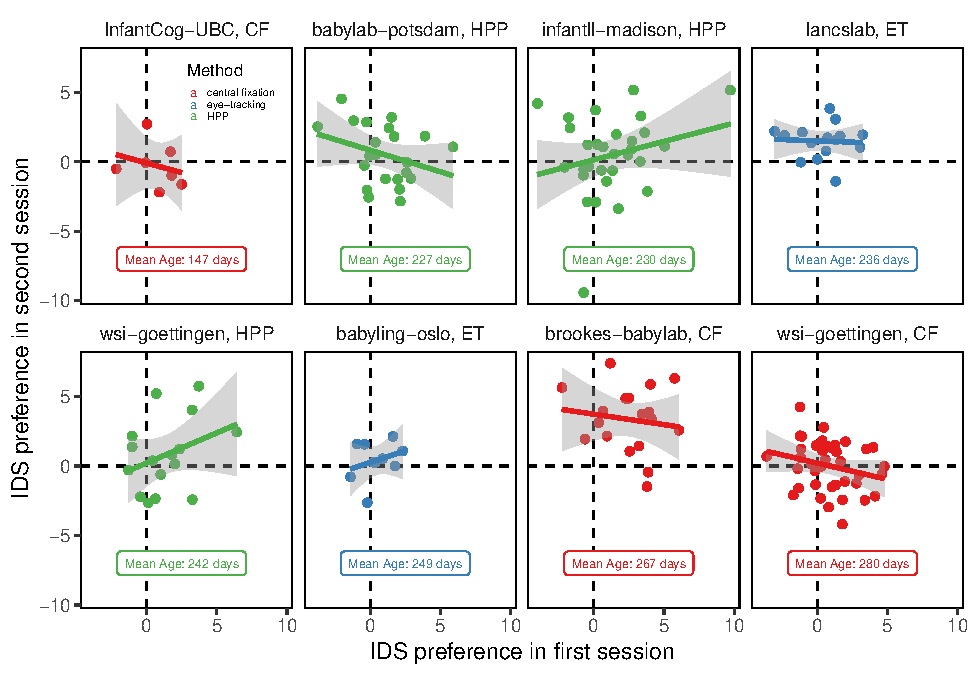
\includegraphics{Retest_current_draft_files/figure-latex/unnamed-chunk-5-1} 

}

\caption{Correlation between IDS Preference in Session 1 and Session 2 in each lab and method. Dots indicate individual participants. Error bands represent 95 percent confidence intervals. The dashed line indicates no preference (i.e., a value of zero) for the first and second session, respectively.}\label{fig:unnamed-chunk-5}
\end{figure}

We assessed test-retest reliability in two planned, confirmatory analyses.
First, we fit a linear mixed-effects model predicting IDS preference in Session 2 from IDS preference in Session 1, including a by-lab random intercept.
The results revealed no significant relationship between IDS preference in Session 1 and 2 (Table 3).
Second, we calculated the Pearson correlation coefficient.
While a simple correlation coefficient might overestimate the test-retest reliability in our sample because it does not control for the differences between different labs and methods (HPP, CF, and ET), we felt it was important to also conduct a Pearson correlation as it is commonly used to assess reliability.
The size of the correlation coefficient was not statistically different from zero and the estimate was small, \(r = .09\), 95\% CI \([-.06, .25]\), \(t(156) = 1.19\), \(p = .237\).
Moreover, no significant correlations emerged in each sample considered separately (Figure 1; see Supplementary Materials S3 for a meta-analytic approach).
41.77\% of the infants reversed their direction of preference for IDS versus ADS from the test to the retest session (see Supplementary Materials S7 for additional analyses of infants' patterns of preferential looking across sessions).

\begin{table}[tbp]

\begin{center}
\begin{threeparttable}

\caption{\label{tab:unnamed-chunk-6}Coefficient estimates from a linear mixed effects model predicting IDS preference in Session 2 and Pearson correlation coefficient for each method separately.}

\begin{tabular}{lllll}
\toprule
Method & $beta$ & $SE$ & $p$ & Pearson $r$\\
\midrule
central fixation & -0.20 & 0.12 & 0.12 & 0.08\\
HPP & 0.15 & 0.14 & 0.28 & 0.13\\
eye-tracking & 0.03 & 0.16 & 0.84 & 0.02\\
\bottomrule
\end{tabular}

\end{threeparttable}
\end{center}

\end{table}

To investigate the test-retest reliability of each specific method, we computed Pearson correlation coefficients and the same mixed-effects model described above for HPP, CF, and ET separately (Table 4) in additional exploratory analyses.
None of the three methods showed evidence of test-retest reliability.
Neither the Pearson correlation coefficients nor the coefficients of the multilevel analysis were significant, all \emph{p}-values \textgreater{} 0.12.
In planned secondary analyses, we found that experimental method, time between test sessions, participant age, and language background did not moderate the relationship between IDS preference in Session 1 and Session 2 (see Supplementary Materials S2).
Taken together, we find no significant evidence of test-retest reliability across our preregistered analyses.

\hypertarget{exploratory-analyses-with-different-inclusion-criteria}{%
\subsection{Exploratory analyses with different inclusion criteria}\label{exploratory-analyses-with-different-inclusion-criteria}}

To this point, all analyses were performed using the inclusion criteria from MB1, which required only that infants contribute at least one trial per condition for inclusion (i.e., one IDS and one ADS trial).
However, more stringent inclusion criteria yielded larger effect sizes in MB1.
We therefore conducted exploratory analyses assessing test-retest reliability after applying progressively stricter inclusion criteria, requiring two, four, six, and eight valid trials per condition.
Applying stricter criteria --- and thereby increasing the number of test trials --- increased reliability numerically from \emph{r} = 0.07 to \emph{r} = 0.34 (Figure 2).
In part due to a decrease in sample size, only one of these correlations was statistically significant (when requiring six trial pairs): two valid trial pairs, \(t(152) = 0.90\), \(p = .367\); four valid trial pairs, \(t(143) = 1.03\), \(p = .306\); six valid trial pairs, \(t(98) = 2.23\), \(p = .028\); eight valid trial pairs --- all trials in both sessions --- \(t(22) = 1.68\), \(p = .108\).
The analyses provide tentative evidence that stricter inclusion criteria may lead to higher test-retest reliability, but at the cost of substantial decreases in sample size (see Supplementary Materials S4 and S6 for additional analyses, including moderator analyses using a more restricted sample).

\begin{figure}

{\centering 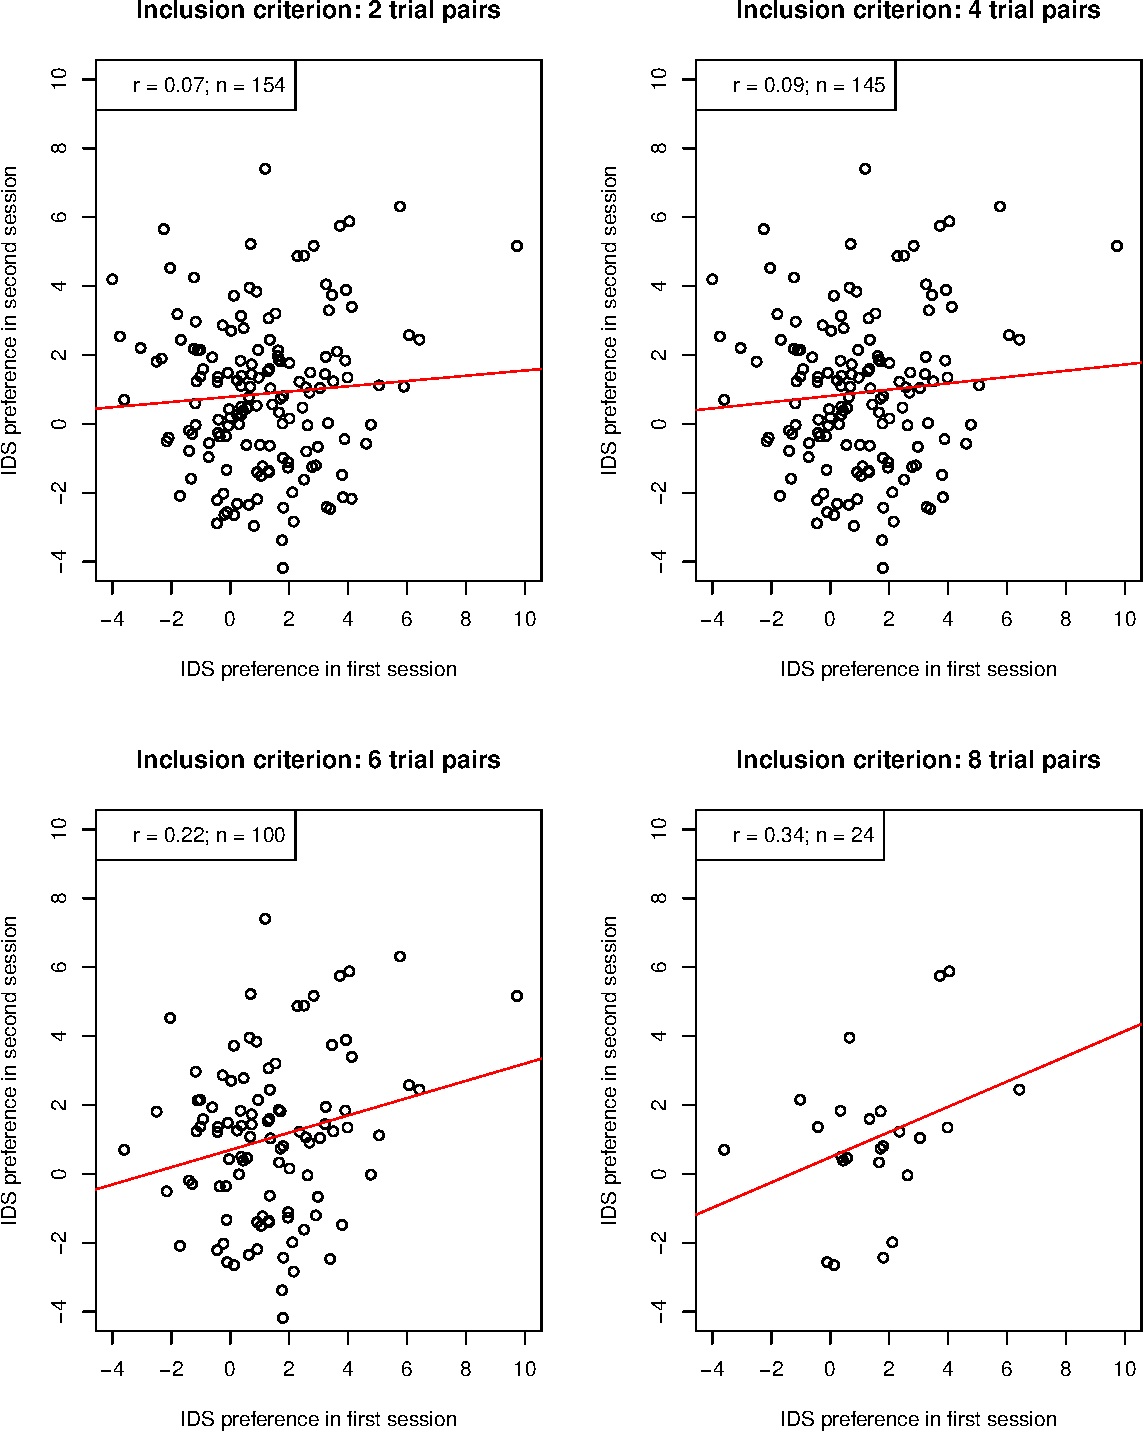
\includegraphics[width=5in]{Retest_current_draft_files/figure-latex/unnamed-chunk-8-1} 

}

\caption{IDS preferences of both sessions plotted against each other for each inclusion criterion. \textit{n} indicates the number of included infants, \textit{r} is the Pearson correlation coefficient as the indicator for reliability.}\label{fig:unnamed-chunk-8}
\end{figure}

\hypertarget{correlations-between-sessions-for-number-of-trials-contributed-and-overall-looking-time}{%
\subsection{Correlations between sessions for number of trials contributed and overall looking time}\label{correlations-between-sessions-for-number-of-trials-contributed-and-overall-looking-time}}

In exploratory analyses, we also investigated whether there were stable individual differences in (a) the number of trials an infant contributed across the two test sessions and (b) infants' overall looking times.

\hypertarget{number-of-trials-contributed}{%
\subsubsection{Number of trials contributed}\label{number-of-trials-contributed}}

We found a strong positive correlation between number of trials contributed during the first and the second session, \(r = .58\), 95\% CI \([.47, .67]\), \(t(160) = 9.00\), \(p < .001\) (Figure 3A).
In other words, if infants contributed a higher number of trials in one session, compared to other infants, they were likely to contribute a higher number of trials in their next session.
This finding is consistent with the hypothesis that how attentive infants are throughout an experiment (and hence how many trials they contribute) is a stable individual difference, at least for some infant looking time tasks.

\hypertarget{overall-looking-times}{%
\subsubsection{Overall looking times}\label{overall-looking-times}}

To what extent are participants looking times between the two sessions related?
To test this question, we investigated whether participants' overall looking times --- irrespective of condition --- were correlated between the first and second session.
There was a robust correlation between average looking time in Session 1 and Session 2: infants with longer looking times during their first session also tended to look longer during their second session, \(r = .45\), 95\% CI \([.31, .57]\), \(t(156) = 6.28\), \(p < .001\) (Figure 3B).
This relationship held even after controlling for number of trials, \(b = 0.42\), 95\% CI \([0.27, 0.58]\), \(t(154) = 5.52\), \(p < .001\), and participants' average age, \(b = 0.44\), 95\% CI \([0.30, 0.59]\), \(t(155) = 6.16\), \(p < .001\), across the two test sessions in linear regression models.
Finally, we found similar correlations in average looking time to IDS stimuli in Session 1 and 2, \(r = .38\), 95\% CI \([.24, .51]\), \(t(156) = 5.19\), \(p < .001\), and ADS stimuli in Session 1 and 2, \(r = .40\), 95\% CI \([.26, .53]\), \(t(156) = 5.49\), \(p < .001\) (Figure 3C; see Supplementary Materials S8 and S9 for further details, including an investigation of item-level correlations).

\begin{figure}

{\centering 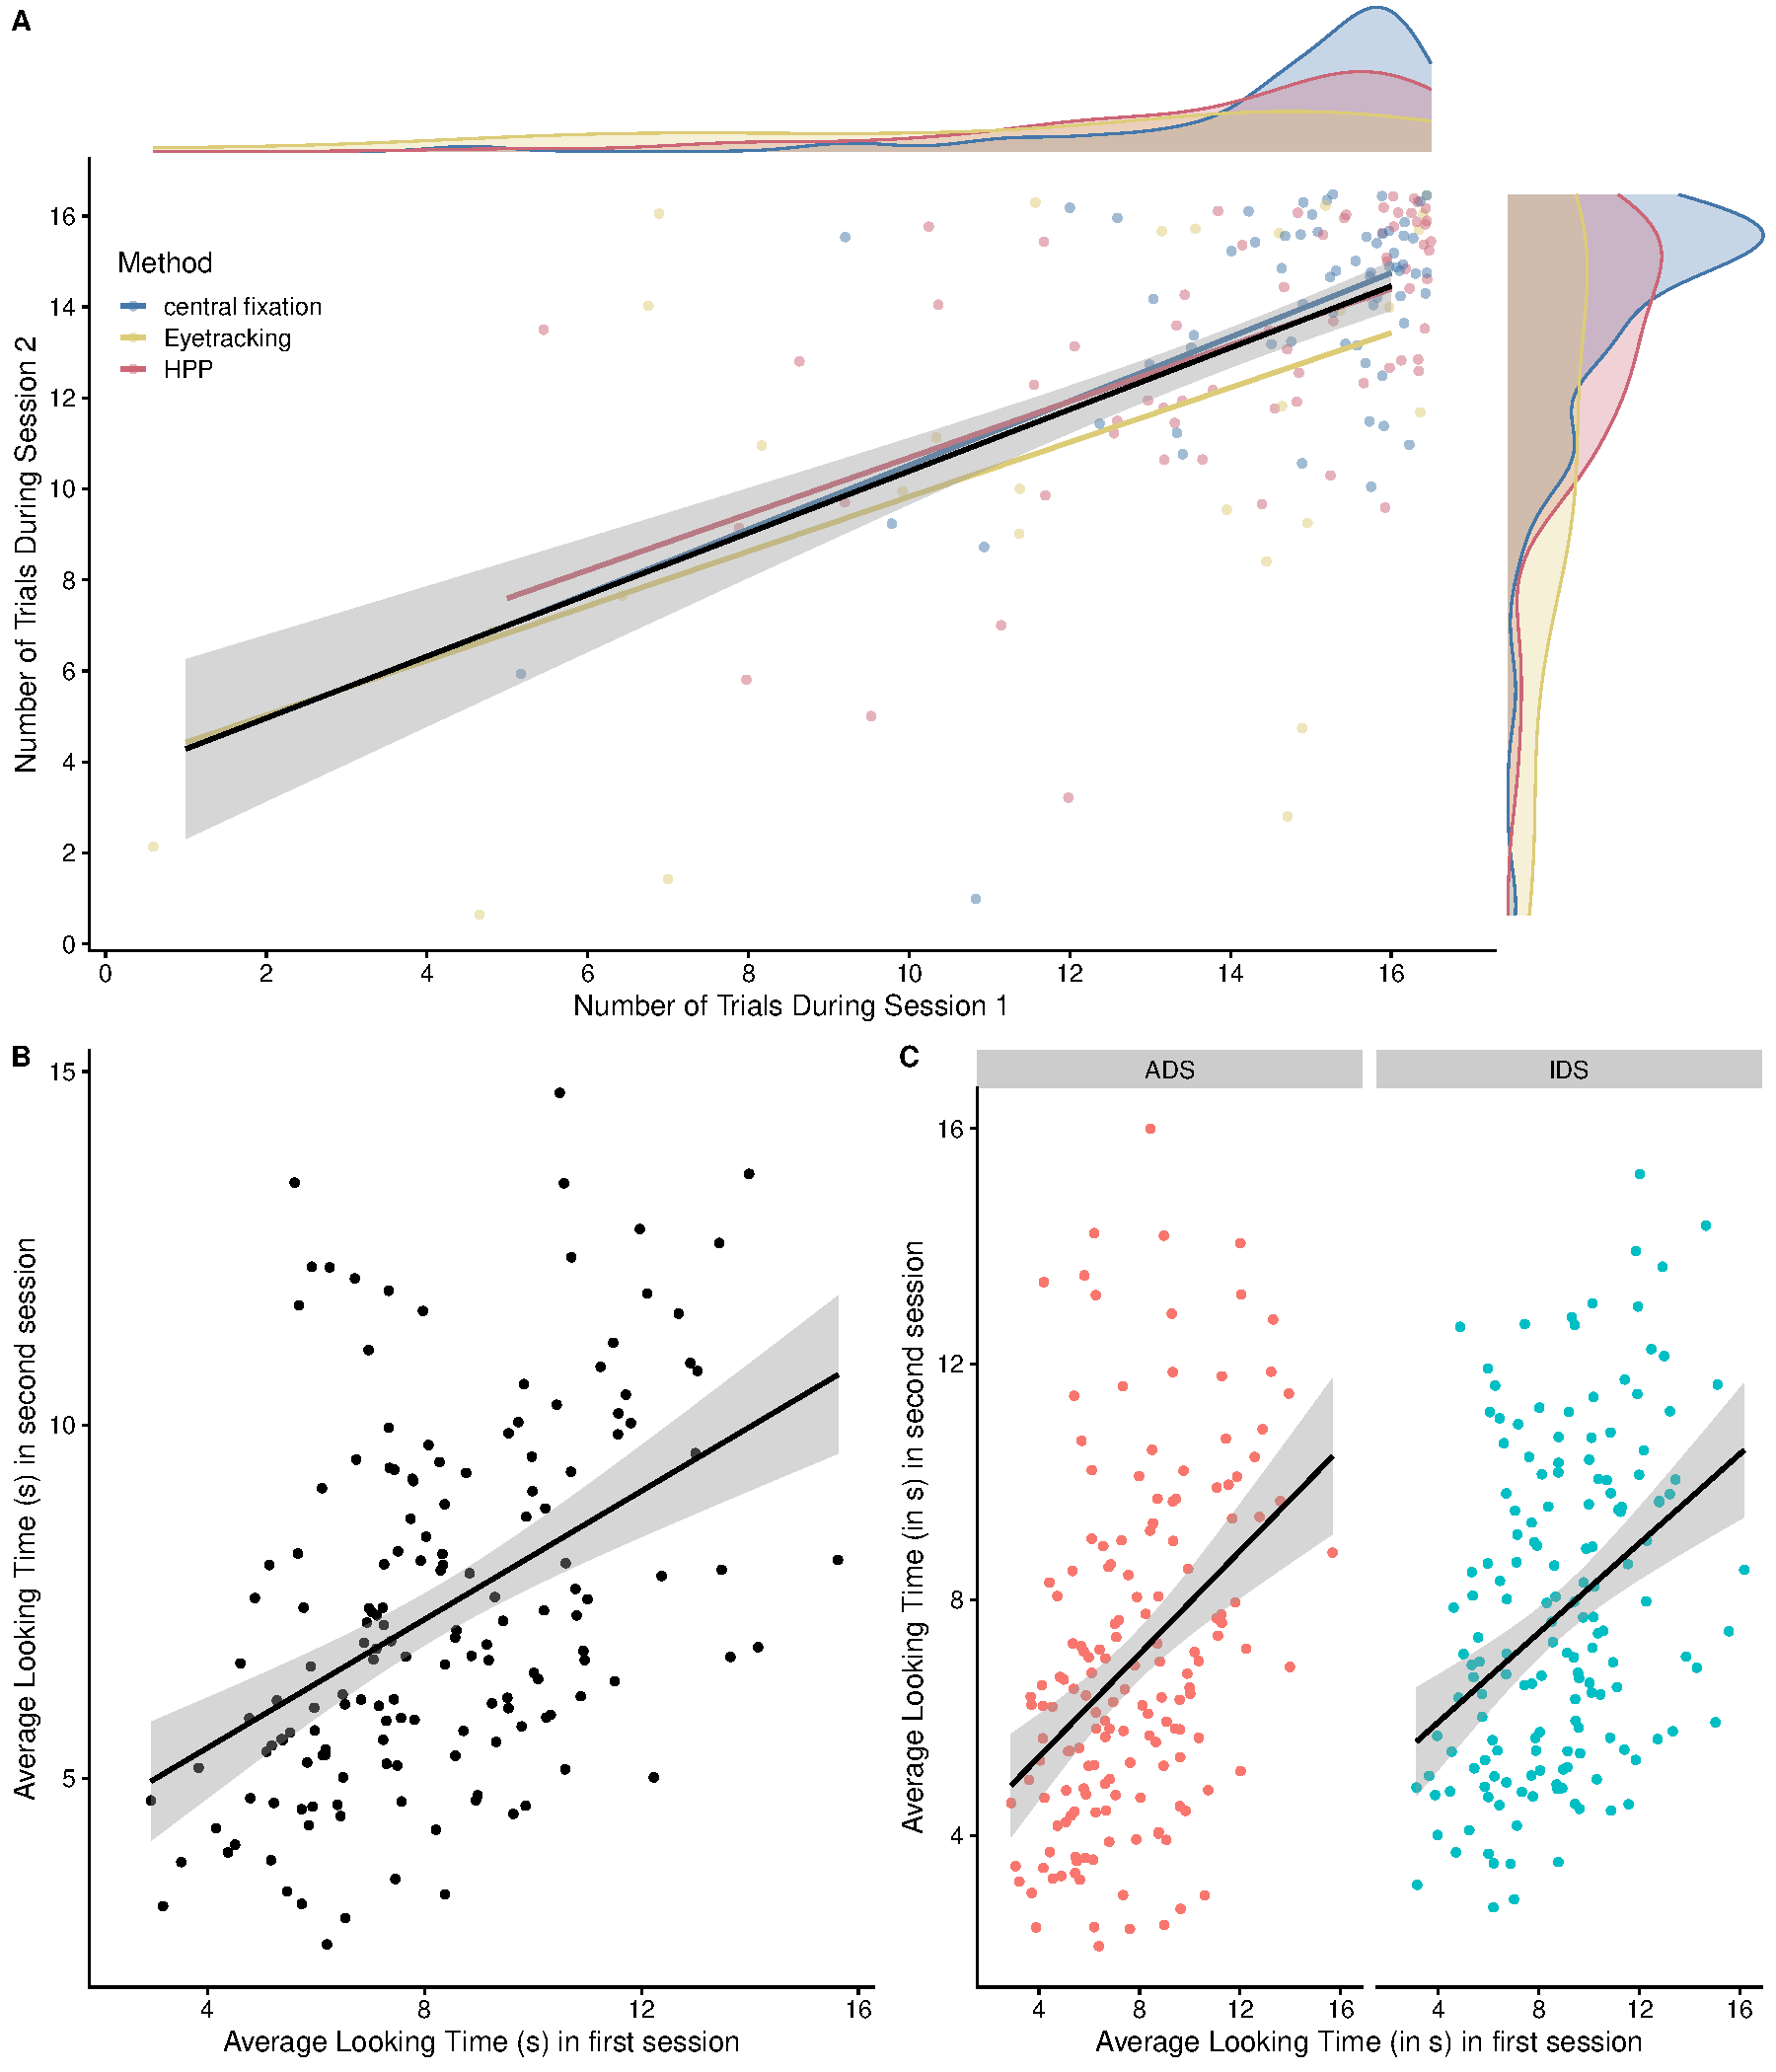
\includegraphics{Retest_current_draft_files/figure-latex/fig3-1} 

}

\caption{(A) Correlation between the number of trials contributed in Session 1 and Session 2. Each data point represents one infant. Colored lines represent linear fits for each method. (B) Overall correlations in average looking time (in s) between Session 1 and 2. (C) Correlations in average looking time (in s) between sessions, split by IDS/ADS condition.}\label{fig:fig3}
\end{figure}

\hypertarget{general-discussion}{%
\section{General Discussion}\label{general-discussion}}

The current study investigated the test-retest reliability of infants' preference for IDS over ADS.
As a spin-off of the original MB1 project, we tested the IDS preference of infants in two separate test sessions to assess the extent to which their pattern of preference would remain consistent.
While we replicated the original effect of infants' speech preference for IDS over ADS for both the test and retest session on the group-level, we found that infants' speech preference measures showed no evidence of test-retest reliability across all preregistered analyses.
In other words, we were unable to find confirmatory evidence of stable individual differences in infants' preference for IDS.
This finding is consistent with past research suggesting low test-retest reliability in other infant paradigms (Cristia et al., 2016; Marimon \& Höhle, 2022).
Given that most experimental procedures conducted in infant research are interested in the comparison of groups, individual differences between participants within a specific condition are usually minimized by the experimental procedure while differences between conditions are maximized.
As a consequence, infant preference measures may be a good approach for capturing group-level phenomena, but may be less appropriate for examining individual differences in development.

We also found no robust evidence that several hypothesized moderators influenced test-retest reliability.
While previous research suggests that HPP may be a more sensitive index of infant preference and speech segmentation abilities (Junge et al., 2020; ManyBabies Consortium, 2020), we found no evidence for higher test-retest reliability for HPP relative to ET and CF.
Similarly, our planned analyses found no evidence that the test-retest reliability of IDS preference varied as a function of the time between test sessions, infants' language background, or infants' age.
The absence of evidence for moderating effects should be treated with caution, given that fewer labs contributed to the study than we had anticipated by the time of the preregistration, resulting in limited power to detect interaction effects (see S2.1 for more detail on power considerations).
However, these analyses also suggest that the lack of test-retest reliability was not be due to variation across any of our hypothesized moderators.

Consistent with general psychometric theory (e.g., DeBolt, Rhemtulla, \& Oakes, 2020), stricter inclusion criteria --- and consequently a larger number of included test trials per participant --- tended to increase the magnitude of the correlation between test sessions.
However, this association was based on exploratory analyses and was in part only observed descriptively, and hence should be interpreted with caution.
A similar effect on the group-level was found in the MB1 project, where a stricter inclusion criterion led to bigger effect sizes (ManyBabies Consortium, 2020).
As in MB1, higher reliability through strict exclusions came at a high cost.
In particular, with the strictest criterion, only a small portion of the original sample size (24 out of 158 infants) could be included in the final sample.
In other words, applying stricter criteria leads to a higher drop-out rate and can dramatically reduce the sample size.
In the case of studies in the field of developmental science, where there are many practical constraints on collecting large samples of infants (e.g., birth rate in the area, restricted lab capacities, budget restrictions), a strict drop-out criterion may often be difficult to implement.
Note that studies in developmental science already have above-average drop-out rates (Miller, 2017).
In addition, drop out is likely not random: the number of trials individual infants contributed was highly correlated between test sessions in the current study.
Therefore, implementing strict inclusion criteria that result in high drop-out rates can further limit the generalizability of a study.
Particularly in the context of turning individual differences measures into diagnostic tools, high drop-out rates have an additional limitation of not being broadly usable.

An alternative approach to increasing the number of valid trials is to increase the number of experimental trials.
This approach seeks to increase the likelihood that participants will contribute sufficient trials (after trial-level exclusions) to allow for precise individual-level estimates (DeBolt et al., 2020; see also Silverstein, Feng, Westermann, Parise, \& Twomey, 2021).
While this approach is promising, it may not always be feasible, because the attention span of a typical infant participant is limited.
Therefore, prolonging the experimental procedure to maximize the absolute number of trials is often challenging in practice.
Other avenues for obtaining higher numbers of valid trials may include changes in the procedure (e.g., Egger, Rowland, \& Bergmann, 2020) or implementing multi-day test sessions (Fernald \& Marchman, 2012), which could become easier with the adoption of online testing methods (Lo, Hermes, Kartushina, Mayor, \& Mani, 2023; Scott \& Schulz, 2017; Weaver, Zettersten, \& Saffran, 2022).

Even under best-case scenarios focused on infants contributing larger numbers of trials, reliability remained low.
For example, when restricting the sample to infants contributing at least 6 trials in each condition in both sessions, we obtained a correlation of \emph{r} = 0.22 and an intra-class correlation coefficient of \(\alpha\) = 0.36.
As Byers-Heinlein et al. (2022) outline, low measurement reliability severely restricts power for detecting relationships between measures.
Using the same approach as Byers-Heinlein et al. (2022), we estimate that over 682 infants would be needed to have at least 80\% power to observe a true correlation of \emph{r} = .3 between two measurements, assuming an intra-class correlation coefficient as large as that observed in our restricted sample (\(\alpha\) = 0.36).
Even a very large true correlation of \emph{r} = .7 would require a sample size of over 120 infants.
In other words, even under optimistic estimates of reliability based on strict inclusion criteria, the low reliability of IDS preference measures would severely limit the feasibility of individual difference and longitudinal research using current methods.

As our results are only based on the phenomenon of IDS preference (albeit, with three widely used methods: HPP, CF, ET), it is essential to further assess the underlying reliability of preferential looking measures within other areas of speech perception (Marimon \& Höhle, 2022).
While most infants prefer IDS over ADS (Dunst et al., 2012), patterns of preferential looking in other tasks (e.g., speech segmentation, artificial grammar learning) are often inconsistent and can vary based on factors such as infants' experience with the testing paradigm (Bergmann \& Cristia, 2016; Santolin, Garcia-Castro, Zettersten, Sebastian-Galles, \& Saffran, 2021).
These inconsistencies in looking behavior are especially important to consider in the context of relating a direction of preference to later language development, and can sometimes lead to seemingly contradictory findings.
That is, both familiarity and novelty responses have been suggested to be predictive of infants' later linguistic abilities (DePaolis, Vihman, \& Keren-Portnoy, 2014; Newman, Ratner, Jusczyk, Jusczyk, \& Dow, 2006; Newman, Rowe, \& Ratner, 2016).
In light of our findings, researchers conducting longitudinal studies with experimental data from young infants predicting future outcomes should be cautious, as there may be large intra-individual variability affecting preference measurement.

While we observed limited evidence for test-retest reliability using preference measures, we observed robust correlations for average looking times between Session 1 and 2, both overall and for IDS and ADS stimuli considered separately (see also Supplementary Materials S8 for an investigation of item-level correlations).
This finding is consistent with past results in infant looking time studies finding robust correlations in average looking times across multiple sessions (Marimon \& Höhle, 2022).
It also raises an apparent puzzle: why are overall looking times for ADS and IDS stimuli correlated, while difference scores are not?
One explanation is that infants have stable individual differences in how long they look to stimuli, but little or no stable individual differences in their preference for one stimulus type over another.
This only partially explains the current pattern of results, however, because IDS looking time in Session 1 predicted IDS looking time in Session 2 even when controlling for ADS looking time, and vice versa (see Supplementary Materials S8).
In other words, the condition-specific looking time correlations are not fully explained by overall looking behavior.
Another long-established explanation is that difference scores tend to have poor measurement reliability, because difference scores combine error from individual measurements into a composite score, increasing the ratio of error relative to the variance between participants (Hedge et al., 2018; Lord, 1956).
Given the limitations of difference scores (and composite scores in general), one goal for future research will be to assess the use of trial-by-trial model-based approaches for estimating reliability (Haines et al., 2020; Rouder \& Haaf, 2019).

\hypertarget{limitations}{%
\subsection{Limitations}\label{limitations}}

While we had an above-average sample size for a study in infant research, we were unable to approach the number of participants collected within the original MB1 study.
Several factors likely contributed to the lower participation rate.
The call to participate in the test-retest spin-off was delayed relative to the MB1 call, scheduling a second lab visit for each participant involved a significant additional effort for participating labs, and there were already other collaborative studies taking place simultaneously (MB1B, Byers-Heinlein, Tsui, Bergmann, et al., 2021; MB1G, Byers-Heinlein, Tsui, Van Renswoude, et al., 2021).
A larger sample size and a greater number of participating labs from different countries would have enabled us to conduct a more highly-powered test of differences in test-retest reliability across different methods, language backgrounds, and participant age.

A further limitation concerns the stimuli.
While the order of the audio recording clips presented to infants within a given trial differed between the first and second session, the exact same stimulus material as in MB1 was used in both sessions.
In particular, all children heard the exact same voices in Session 1 and in Session 2.
From a practical point of view, this was the most straightforward solution for coordinating the experiment within the larger MB1 project.
However, familiarity effects might have influenced infants' looking behavior.
Infants with longer looking times in their first session might have had more opportunity to recognize familiar audio clips in their second session.
For infants with short looking times, familiar audio clips would only occur towards the end of second-session trials, thus offering infants less opportunity to recognize voices from their first session.
Therefore, inconsistent familiarity with the stimulus material in the second session across infants might have artificially lowered test-retest reliability.
However, in supplementary analyses, we found that test-retest reliability was not significantly moderated by infants' overall looking time during their first testing session (see Supplementary Materials S10).
Moreover, infants' looking times generally declined in Session 2 compared to Session 1 (consistent with past work, e.g., Marimon \& Höhle, 2022), limiting opportunities for infants to encounter previously experienced stimulus material.

\hypertarget{conclusion}{%
\section{Conclusion}\label{conclusion}}

Following the MB1 protocol, the current study could not detect test-retest reliability in measures of infants' preference for IDS over ADS.
Subsequent analyses provided tentative evidence that stricter criteria for the inclusion of participants may enhance test-retest reliability at the cost of high drop-out rates.
Developmental studies relying on stable individual differences between their participants need to consider the underlying reliability of their measures, and we recommend a broader assessment of test-retest reliability in infant research.

\newpage

\hypertarget{references}{%
\section{References}\label{references}}

\begingroup
\setlength{\parindent}{-0.5in}
\setlength{\leftskip}{0.5in}

\hypertarget{refs}{}
\begin{CSLReferences}{1}{0}
\leavevmode\vadjust pre{\hypertarget{ref-bergmann2016development}{}}%
Bergmann, C., \& Cristia, A. (2016). Development of infants' segmentation of words from native speech: A meta-analytic approach. \emph{Developmental Science}, \emph{19}(6), 901--917.

\leavevmode\vadjust pre{\hypertarget{ref-byers2021six}{}}%
Byers-Heinlein, K., Bergmann, C., \& Savalei, V. (2022). Six solutions for more reliable infant research. \emph{Infant and Child Development}, \emph{31}(5), e2296.

\leavevmode\vadjust pre{\hypertarget{ref-byers2021multilab}{}}%
Byers-Heinlein, K., Tsui, A. S. M., Bergmann, C., Black, A. K., Brown, A., Carbajal, M. J., \ldots{} Wermelinger, S. (2021). A multilab study of bilingual infants: Exploring the preference for infant-directed speech. \emph{Advances in Methods and Practices in Psychological Science}, \emph{4}(1), 2515245920974622.

\leavevmode\vadjust pre{\hypertarget{ref-byers2021development}{}}%
Byers-Heinlein, K., Tsui, R. K.-Y., Van Renswoude, D., Black, A. K., Barr, R., Brown, A., \ldots{} Singh, L. (2021). The development of gaze following in monolingual and bilingual infants: A multi-laboratory study. \emph{Infancy}, \emph{26}(1), 4--38.

\leavevmode\vadjust pre{\hypertarget{ref-colombo1988infant}{}}%
Colombo, J., Mitchell, D. W., \& Horowitz, F. D. (1988). Infant visual attention in the paired-comparison paradigm: Test-retest and attention-performance relations. \emph{Child Development}, 1198--1210.

\leavevmode\vadjust pre{\hypertarget{ref-cooper1990preference}{}}%
Cooper, R. P., \& Aslin, R. N. (1990). Preference for infant-directed speech in the first month after birth. \emph{Child Development}, \emph{61}(5), 1584--1595.

\leavevmode\vadjust pre{\hypertarget{ref-cristia2014predicting}{}}%
Cristia, A., Seidl, A., Junge, C., Soderstrom, M., \& Hagoort, P. (2014). Predicting individual variation in language from infant speech perception measures. \emph{Child Development}, \emph{85}(4), 1330--1345.

\leavevmode\vadjust pre{\hypertarget{ref-cristia2016test}{}}%
Cristia, A., Seidl, A., Singh, L., \& Houston, D. (2016). Test--retest reliability in infant speech perception tasks. \emph{Infancy}, \emph{21}(5), 648--667.

\leavevmode\vadjust pre{\hypertarget{ref-debolt2020robust}{}}%
DeBolt, M. C., Rhemtulla, M., \& Oakes, L. M. (2020). Robust data and power in infant research: A case study of the effect of number of infants and number of trials in visual preference procedures. \emph{Infancy}, \emph{25}(4), 393--419.

\leavevmode\vadjust pre{\hypertarget{ref-depaolis2014infants}{}}%
DePaolis, R. A., Vihman, M. M., \& Keren-Portnoy, T. (2014). When do infants begin recognizing familiar words in sentences? \emph{Journal of Child Language}, \emph{41}(1), 226--239.

\leavevmode\vadjust pre{\hypertarget{ref-dunst2012preference}{}}%
Dunst, C., Gorman, E., \& Hamby, D. (2012). Preference for infant-directed speech in preverbal young children. \emph{Center for Early Literacy Learning}, \emph{5}(1), 1--13. Retrieved from \url{http://www.earlyliteracylearning.org/cellreviews/cellreviews_v5_n1.pdf}

\leavevmode\vadjust pre{\hypertarget{ref-egger2020improving}{}}%
Egger, J., Rowland, C. F., \& Bergmann, C. (2020). Improving the robustness of infant lexical processing speed measures. \emph{Behavior Research Methods}, \emph{52}(5), 2188--2201.

\leavevmode\vadjust pre{\hypertarget{ref-fernald2012individual}{}}%
Fernald, A., \& Marchman, V. A. (2012). Individual differences in lexical processing at 18 months predict vocabulary growth in typically developing and late-talking toddlers. \emph{Child Development}, \emph{83}(1), 203--222.

\leavevmode\vadjust pre{\hypertarget{ref-fernald1989cross}{}}%
Fernald, A., Taeschner, T., Dunn, J., Papousek, M., Boysson-Bardies, B. de, \& Fukui, I. (1989). A cross-language study of prosodic modifications in mothers' and fathers' speech to preverbal infants. \emph{Journal of Child Language}, \emph{16}(3), 477--501.

\leavevmode\vadjust pre{\hypertarget{ref-floccia2016british}{}}%
Floccia, C., Keren-Portnoy, T., DePaolis, R., Duffy, H., Delle Luche, C., Durrant, S., \ldots{} Vihman, M. (2016). British english infants segment words only with exaggerated infant-directed speech stimuli. \emph{Cognition}, \emph{148}, 1--9.

\leavevmode\vadjust pre{\hypertarget{ref-frank2017collaborative}{}}%
Frank, M. C., Bergelson, E., Bergmann, C., Cristia, A., Floccia, C., Gervain, J., \ldots{} Yurovsky, D. (2017). A collaborative approach to infant research: Promoting reproducibility, best practices, and theory-building. \emph{Infancy}, \emph{22}(4), 421--435. \url{https://doi.org/10.1111/infa.12182}

\leavevmode\vadjust pre{\hypertarget{ref-graf2013infant}{}}%
Graf Estes, K., \& Hurley, K. (2013). Infant-directed prosody helps infants map sounds to meanings. \emph{Infancy}, \emph{18}(5), 797--824. \url{https://doi.org/10.1111/infa.12006}

\leavevmode\vadjust pre{\hypertarget{ref-haines_theoretically_2020}{}}%
Haines, N., Kvam, P. D., Irving, L. H., Smith, C., Beauchaine, T. P., Pitt, M. A., \ldots{} Turner, B. (2020). \emph{Theoretically {Informed} {Generative} {Models} {Can} {Advance} the {Psychological} and {Brain} {Sciences}: {Lessons} from the {Reliability} {Paradox}} {[}Preprint{]}. PsyArXiv. \url{https://doi.org/10.31234/osf.io/xr7y3}

\leavevmode\vadjust pre{\hypertarget{ref-hedge2018reliability}{}}%
Hedge, C., Powell, G., \& Sumner, P. (2018). The reliability paradox: Why robust cognitive tasks do not produce reliable individual differences. \emph{Behavior Research Methods}, \emph{50}(3), 1166--1186.

\leavevmode\vadjust pre{\hypertarget{ref-houston2007assessing}{}}%
Houston, D. M., Horn, D. L., Qi, R., Ting, J. Y., \& Gao, S. (2007). Assessing speech discrimination in individual infants. \emph{Infancy}, \emph{12}(2), 119--145.

\leavevmode\vadjust pre{\hypertarget{ref-hunter1988multifactor}{}}%
Hunter, M. A., \& Ames, E. W. (1988). A multifactor model of infant preferences for novel and familiar stimuli. \emph{Advances in Infancy Research}, \emph{5}, 69--95.

\leavevmode\vadjust pre{\hypertarget{ref-johnson2010using}{}}%
Johnson, E., \& Zamuner, T. (2010). Using infant and toddler testing methods in language acquisition research. In E. Blom \& S. Unsworth (Eds.), \emph{Experimental methods in language acquisition research} (pp. 73--93). Amsterdam: John Benjamins Publishing Company.

\leavevmode\vadjust pre{\hypertarget{ref-junge2020contrasting}{}}%
Junge, C., Everaert, E., Porto, L., Fikkert, P., Klerk, M. de, Keij, B., \& Benders, T. (2020). Contrasting behavioral looking procedures: A case study on infant speech segmentation. \emph{Infant Behavior and Development}, \emph{60}, 101448.

\leavevmode\vadjust pre{\hypertarget{ref-lo_e-babylab_2023}{}}%
Lo, C. H., Hermes, J., Kartushina, N., Mayor, J., \& Mani, N. (2023). E-{Babylab}: {An} open-source browser-based tool for unmoderated online developmental studies. \emph{Behavior Research Methods}. \url{https://doi.org/10.3758/s13428-023-02200-7}

\leavevmode\vadjust pre{\hypertarget{ref-lord_measurement_growth}{}}%
Lord, F. M. (1956). The measurement of growth. \emph{Educational and Psychological Measurement}, \emph{16}, 421--437. \url{https://doi.org/10.1177/001316445601600401}

\leavevmode\vadjust pre{\hypertarget{ref-ma2011word}{}}%
Ma, W., Golinkoff, R. M., Houston, D. M., \& Hirsh-Pasek, K. (2011). Word learning in infant-and adult-directed speech. \emph{Language Learning and Development}, \emph{7}(3), 185--201.

\leavevmode\vadjust pre{\hypertarget{ref-manybabies2020quantifying}{}}%
ManyBabies Consortium. (2020). Quantifying sources of variability in infancy research using the infant-directed-speech preference. \emph{Advances in Methods and Practices in Psychological Science}, \emph{3}(1), 24--52.

\leavevmode\vadjust pre{\hypertarget{ref-marimon2022}{}}%
Marimon, M., \& Höhle, B. (2022). Testing prosodic development with the headturn preference procedure: A test-retest reliability study. \emph{Infant and Child Development}, e2362.

\leavevmode\vadjust pre{\hypertarget{ref-miller2017developmental}{}}%
Miller, S. A. (2017). \emph{Developmental research methods}. Sage publications.

\leavevmode\vadjust pre{\hypertarget{ref-naoi2012cerebral}{}}%
Naoi, N., Minagawa-Kawai, Y., Kobayashi, A., Takeuchi, K., Nakamura, K., Yamamoto, J., \& Shozo, K. (2012). Cerebral responses to infant-directed speech and the effect of talker familiarity. \emph{Neuroimage}, \emph{59}(2), 1735--1744.

\leavevmode\vadjust pre{\hypertarget{ref-newman2006infants}{}}%
Newman, R., Ratner, N. B., Jusczyk, A. M., Jusczyk, P. W., \& Dow, K. A. (2006). Infants' early ability to segment the conversational speech signal predicts later language development: A retrospective analysis. \emph{Developmental Psychology}, \emph{42}(4), 643.

\leavevmode\vadjust pre{\hypertarget{ref-newman2016input}{}}%
Newman, R., Rowe, M. L., \& Ratner, N. B. (2016). Input and uptake at 7 months predicts toddler vocabulary: The role of child-directed speech and infant processing skills in language development. \emph{Journal of Child Language}, \emph{43}(5), 1158--1173.

\leavevmode\vadjust pre{\hypertarget{ref-oakes2017sample}{}}%
Oakes, L. M. (2017). Sample size, statistical power, and false conclusions in infant looking-time research. \emph{Infancy}, \emph{22}(4), 436--469.

\leavevmode\vadjust pre{\hypertarget{ref-oliveira_reliability_2023}{}}%
Oliveira, C. M., Hayiou-Thomas, M. E., \& Henderson, L. M. (2023). The reliability of the serial reaction time task: Meta-analysis of test--retest correlations. \emph{Royal Society Open Science}, \emph{10}(7), 221542. \url{https://doi.org/10.1098/rsos.221542}

\leavevmode\vadjust pre{\hypertarget{ref-rouder_psychometrics_2019}{}}%
Rouder, J. N., \& Haaf, J. M. (2019). A psychometrics of individual differences in experimental tasks. \emph{Psychonomic Bulletin \& Review}, \emph{26}(2), 452--467. \url{https://doi.org/10.3758/s13423-018-1558-y}

\leavevmode\vadjust pre{\hypertarget{ref-santolin_experience_2021}{}}%
Santolin, C., Garcia-Castro, G., Zettersten, M., Sebastian-Galles, N., \& Saffran, J. R. (2021). Experience with research paradigms relates to infants' direction of preference. \emph{Infancy}, \emph{26}(1), 39--46. \url{https://doi.org/10.1111/infa.12372}

\leavevmode\vadjust pre{\hypertarget{ref-schreiner2017listen}{}}%
Schreiner, M. S., \& Mani, N. (2017). Listen up! Developmental differences in the impact of IDS on speech segmentation. \emph{Cognition}, \emph{160}, 98--102.

\leavevmode\vadjust pre{\hypertarget{ref-lookit2017_1}{}}%
Scott, K. M., \& Schulz, L. E. (2017). Lookit (part 1): A new online platform for developmental research. \emph{Open Mind}, \emph{1}(1), 4--14. \url{https://doi.org/doi:10.1162/opmi_a_00002}

\leavevmode\vadjust pre{\hypertarget{ref-silverstein2021infants}{}}%
Silverstein, P., Feng, J., Westermann, G., Parise, E., \& Twomey, K. E. (2021). Infants learn to follow gaze in stages: Evidence confirming a robotic prediction. \emph{Open Mind}, 1--15.

\leavevmode\vadjust pre{\hypertarget{ref-singh2009influences}{}}%
Singh, L., Nestor, S., Parikh, C., \& Yull, A. (2009). Influences of infant-directed speech on early word recognition. \emph{Infancy}, \emph{14}(6), 654--666.

\leavevmode\vadjust pre{\hypertarget{ref-thiessen2005infant}{}}%
Thiessen, E. D., Hill, E. A., \& Saffran, J. R. (2005). Infant-directed speech facilitates word segmentation. \emph{Infancy}, \emph{7}(1), 53--71. \url{https://doi.org/10.1207/s15327078in0701_5}

\leavevmode\vadjust pre{\hypertarget{ref-weaver_2022}{}}%
Weaver, H., Zettersten, M., \& Saffran, J. (2022). \emph{Becoming word meaning experts: Infants' processing of familiar words in the context of typical and atypical exemplars.} {[}Preprint{]}. PsyArXiv. \url{https://doi.org/10.31234/osf.io/njh38}

\leavevmode\vadjust pre{\hypertarget{ref-zangl2007increased}{}}%
Zangl, R., \& Mills, D. L. (2007). Increased brain activity to infant-directed speech in 6-and 13-month-old infants. \emph{Infancy}, \emph{11}(1), 31--62. \url{https://doi.org/10.1207/s15327078in1101_2}

\end{CSLReferences}

\endgroup


\end{document}
